\section{文献管理软件}
\subsection{介绍}

写论文最好有一个文献管理软件,方便管理参考文献。常用的有 EndNote、Mendeley、Zotero 等。
我们学校已经购买了 Endnote 正版授权,可以到\textbf{\textcolor{blue}{\href{https://zbhrj1.jlu.edu.cn/download/EndNote21W.html}{吉大正版网站}}}下载使用。
但是界面是全英文的,使用操作也不符合我的习惯,我这里只介绍我在用的Zotero,使用应该大同小异。



\subsection{下载安装}

Zotero基础功能免费,高级功能(如大容量云盘同步)是需要付费的,不过我们基本只用得到免费功能。
软件可以在\textbf{\textcolor{blue}{\href{https://www.zotero.org/}{Zotero官方网站}}}直接下载使用。

安装过程与一般软件类似,看不懂就直接下一步。

\subsection{文献导入方法}

提示:下面图片看不清可以放大,理论上清晰度是足够的。

打开软件后,在“我的文库”右键,可以新建分类:

\begin{figure}[htbp]
    \centering
    \captionsetup{font={small, bf}, margin=60pt}
    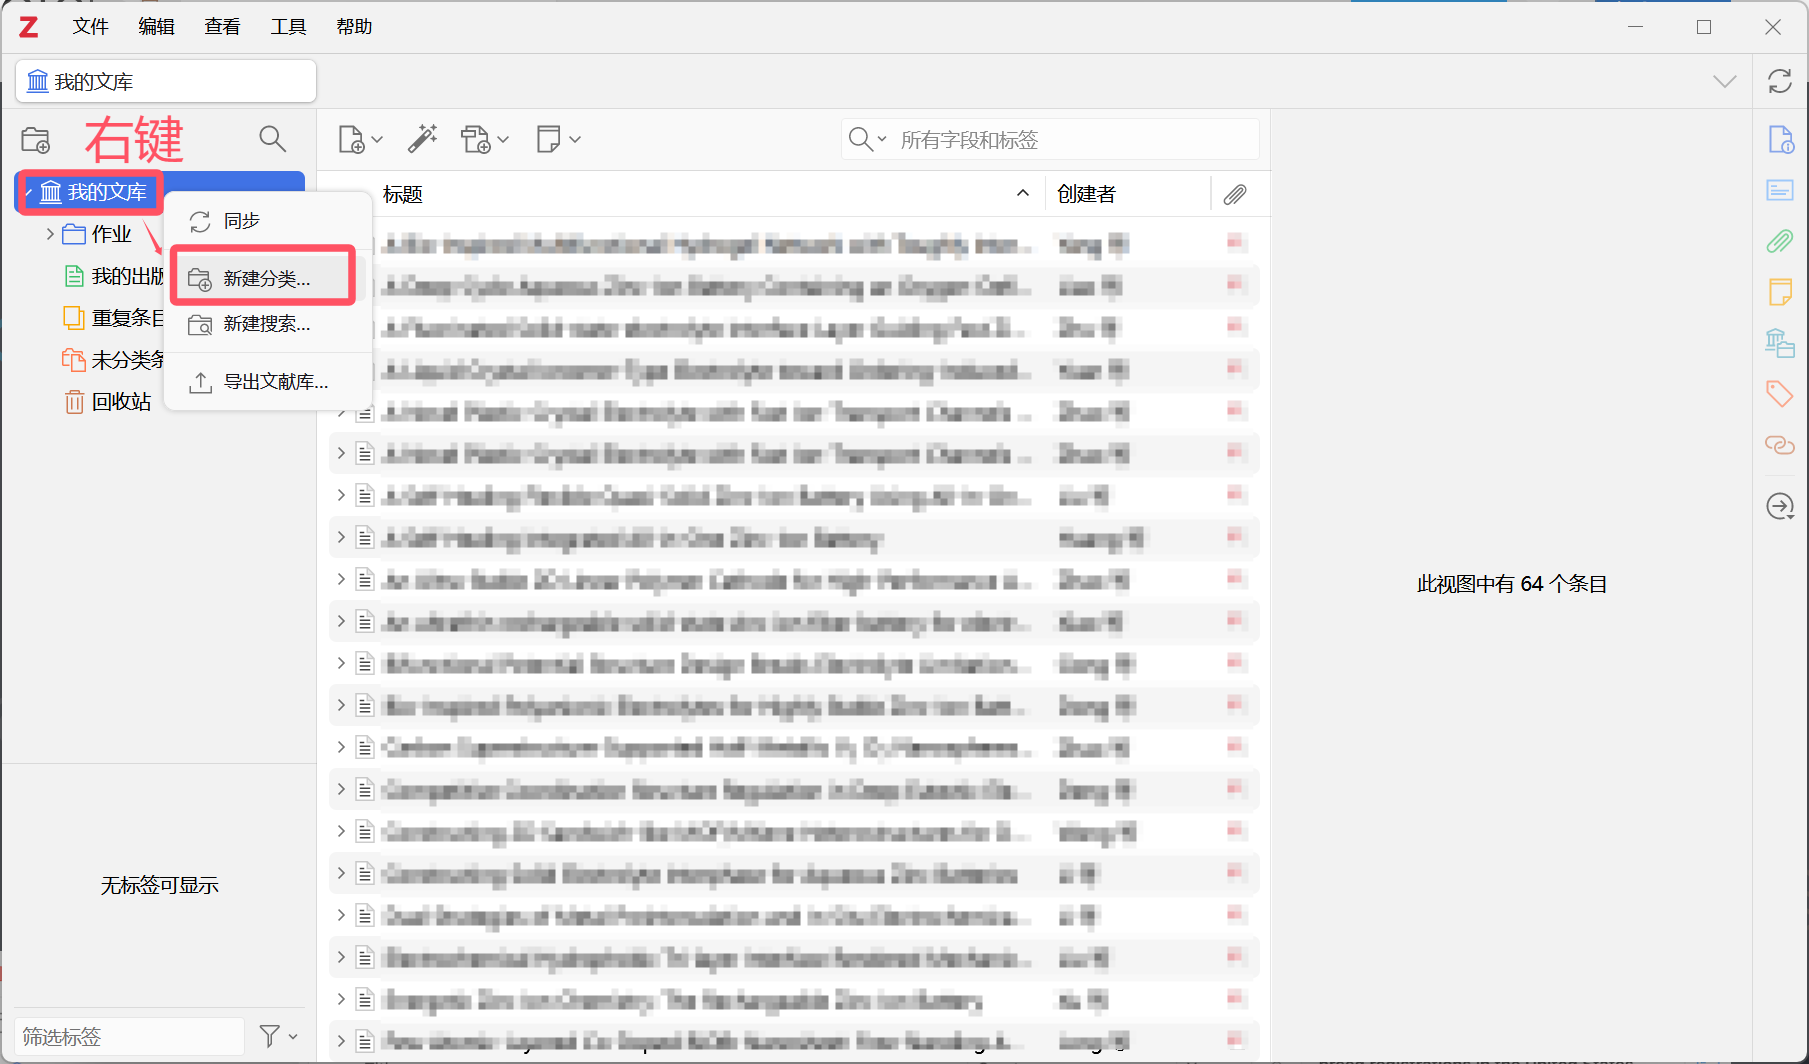
\includegraphics[width=0.8\textwidth]{Zotero打开.png}
    \caption{Zotero}
    \label{Zotero 1}
\end{figure}

\newpage

之后可直接拖拽文献PDF导入:

\begin{figure}[htbp]
    \centering
    \captionsetup{font={small, bf}, margin=60pt}
    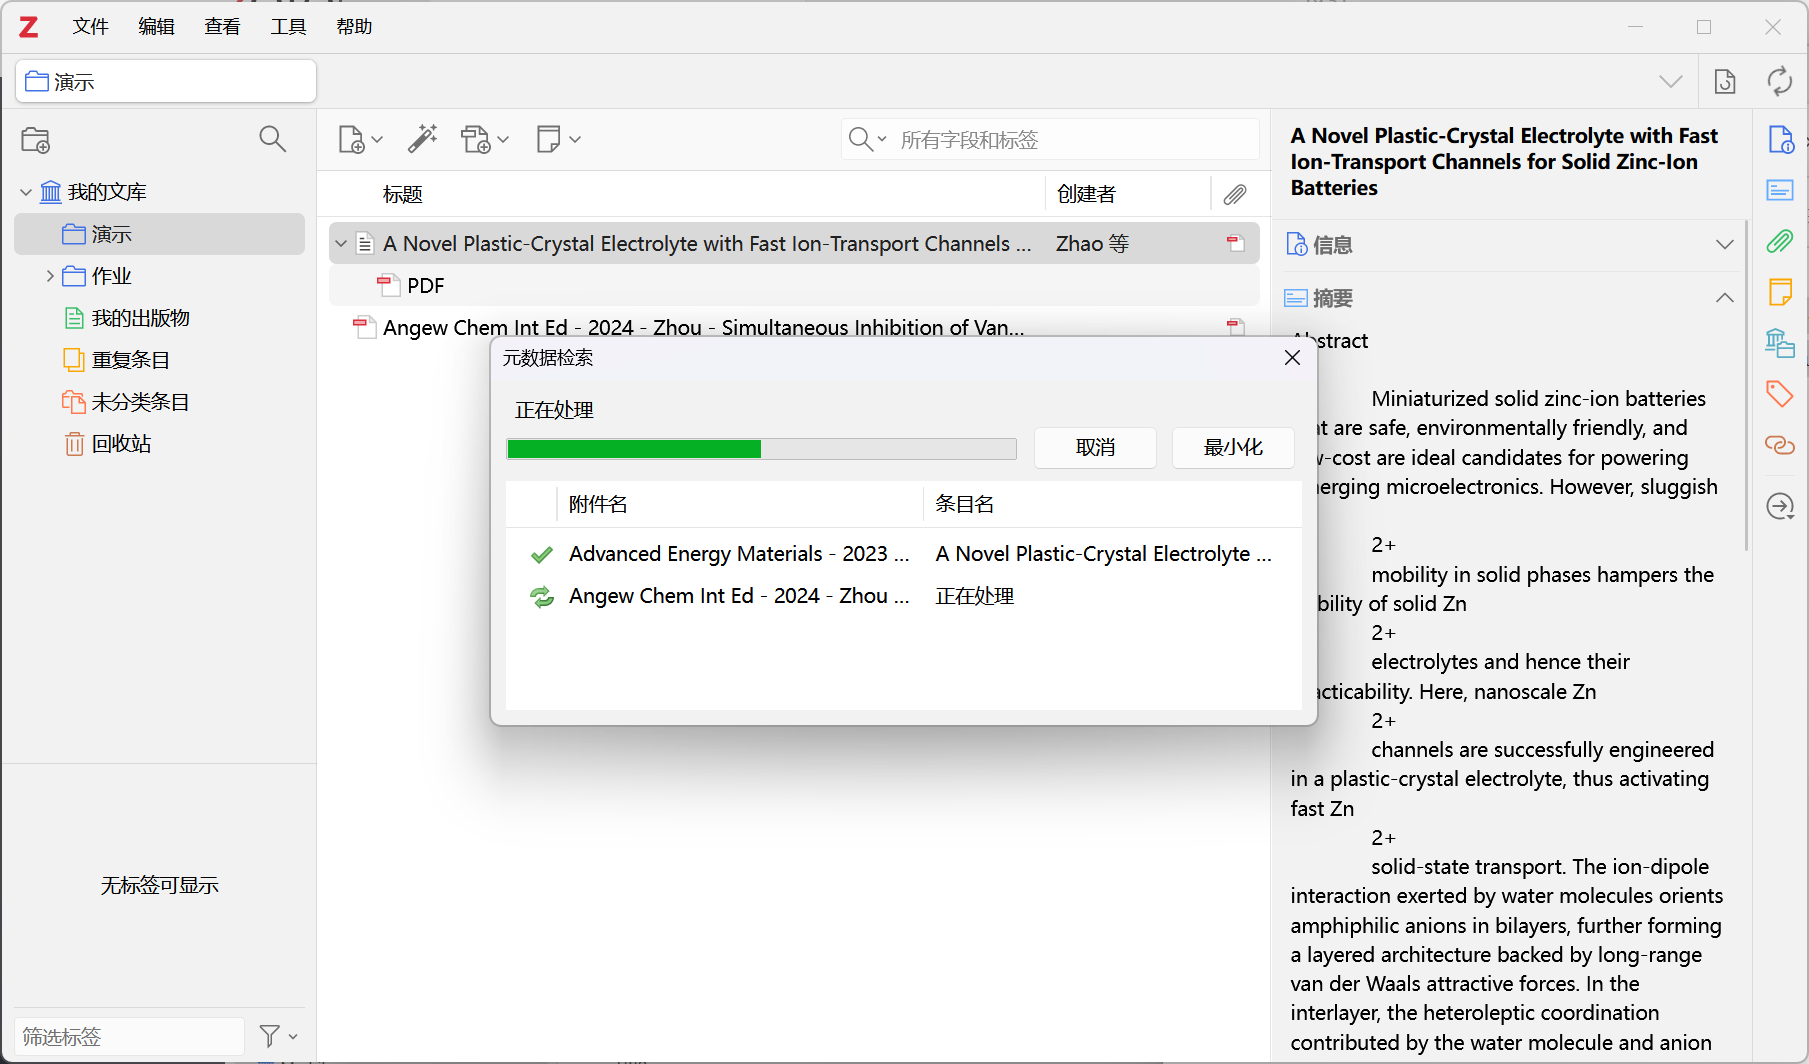
\includegraphics[width=0.8\textwidth]{Zotero导入.png}
    \caption{Zotero}
    \label{Zotero 2}
\end{figure}

也可以安装浏览器拓展直接在浏览器导入:
\begin{figure}[h]
    \centering
    \captionsetup{font={small, bf}, margin=60pt}
    \begin{subfigure}[c]{0.48\textwidth}
      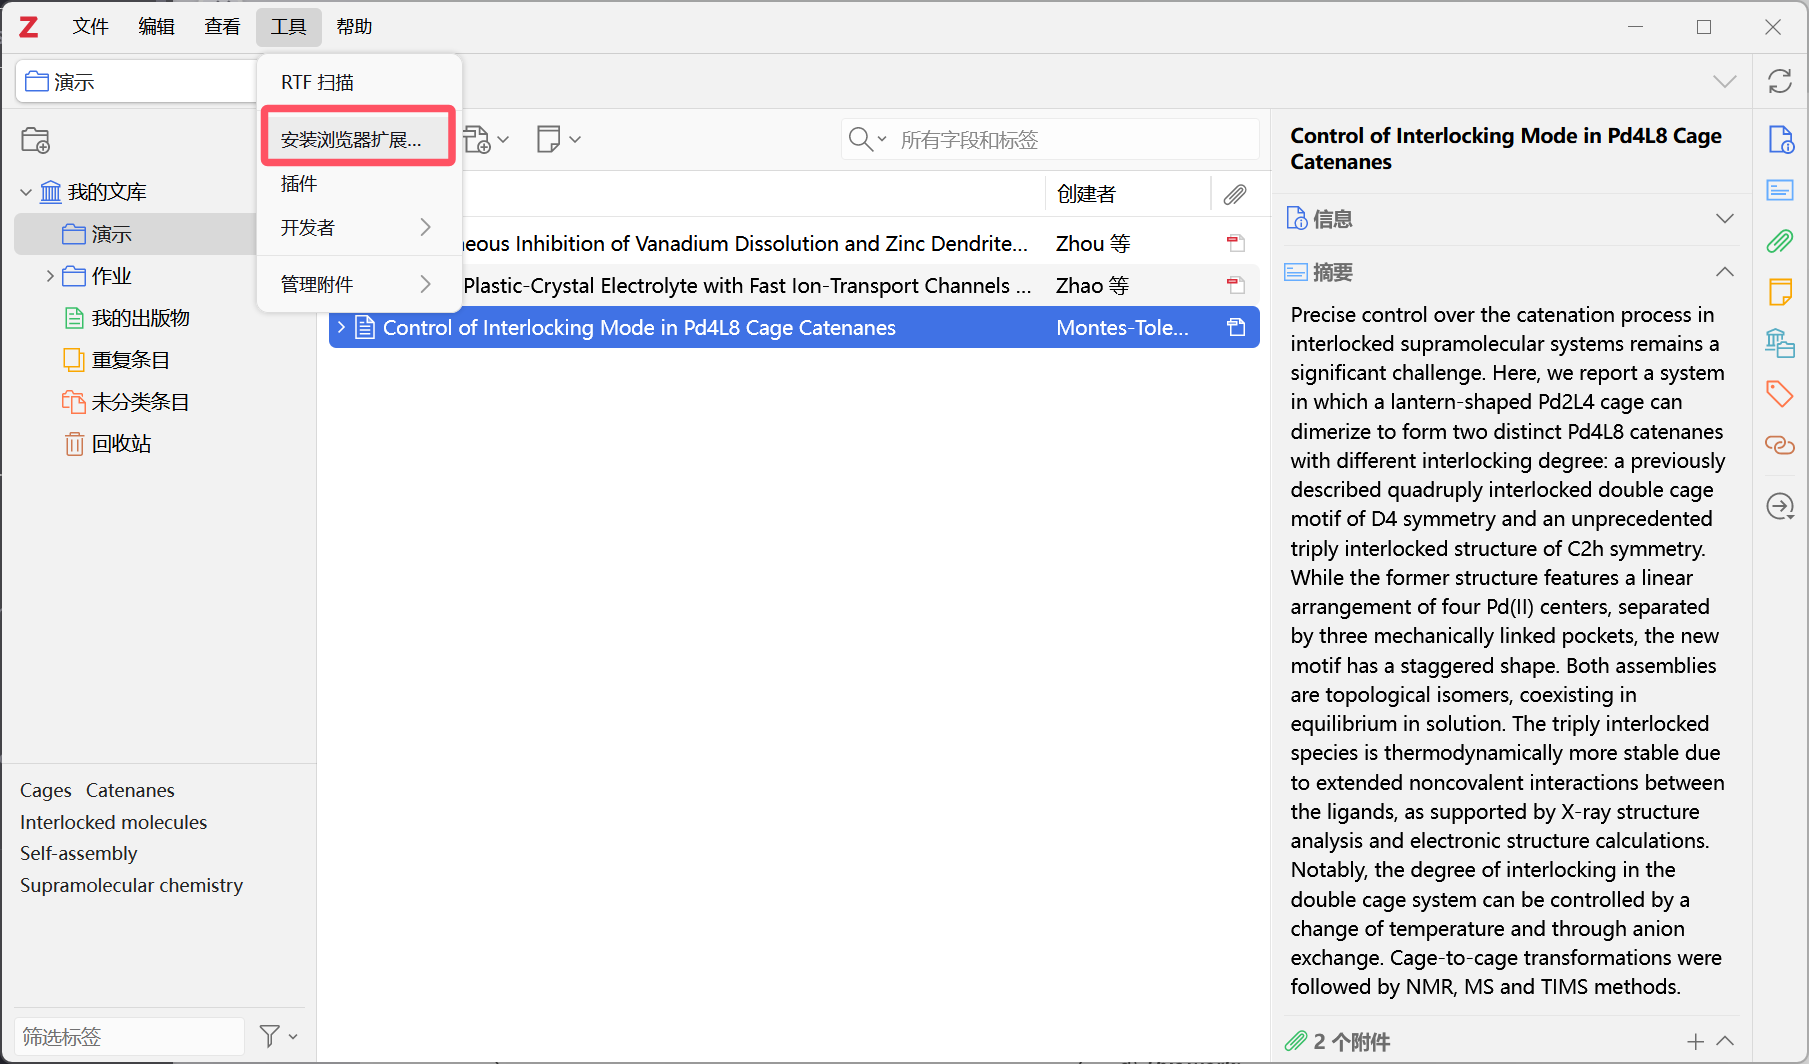
\includegraphics[width=\textwidth]{浏览器拓展安装.png}
      \label{Zotero 3-1}
    \end{subfigure}
    \hfill
    \begin{subfigure}[c]{0.48\textwidth}
      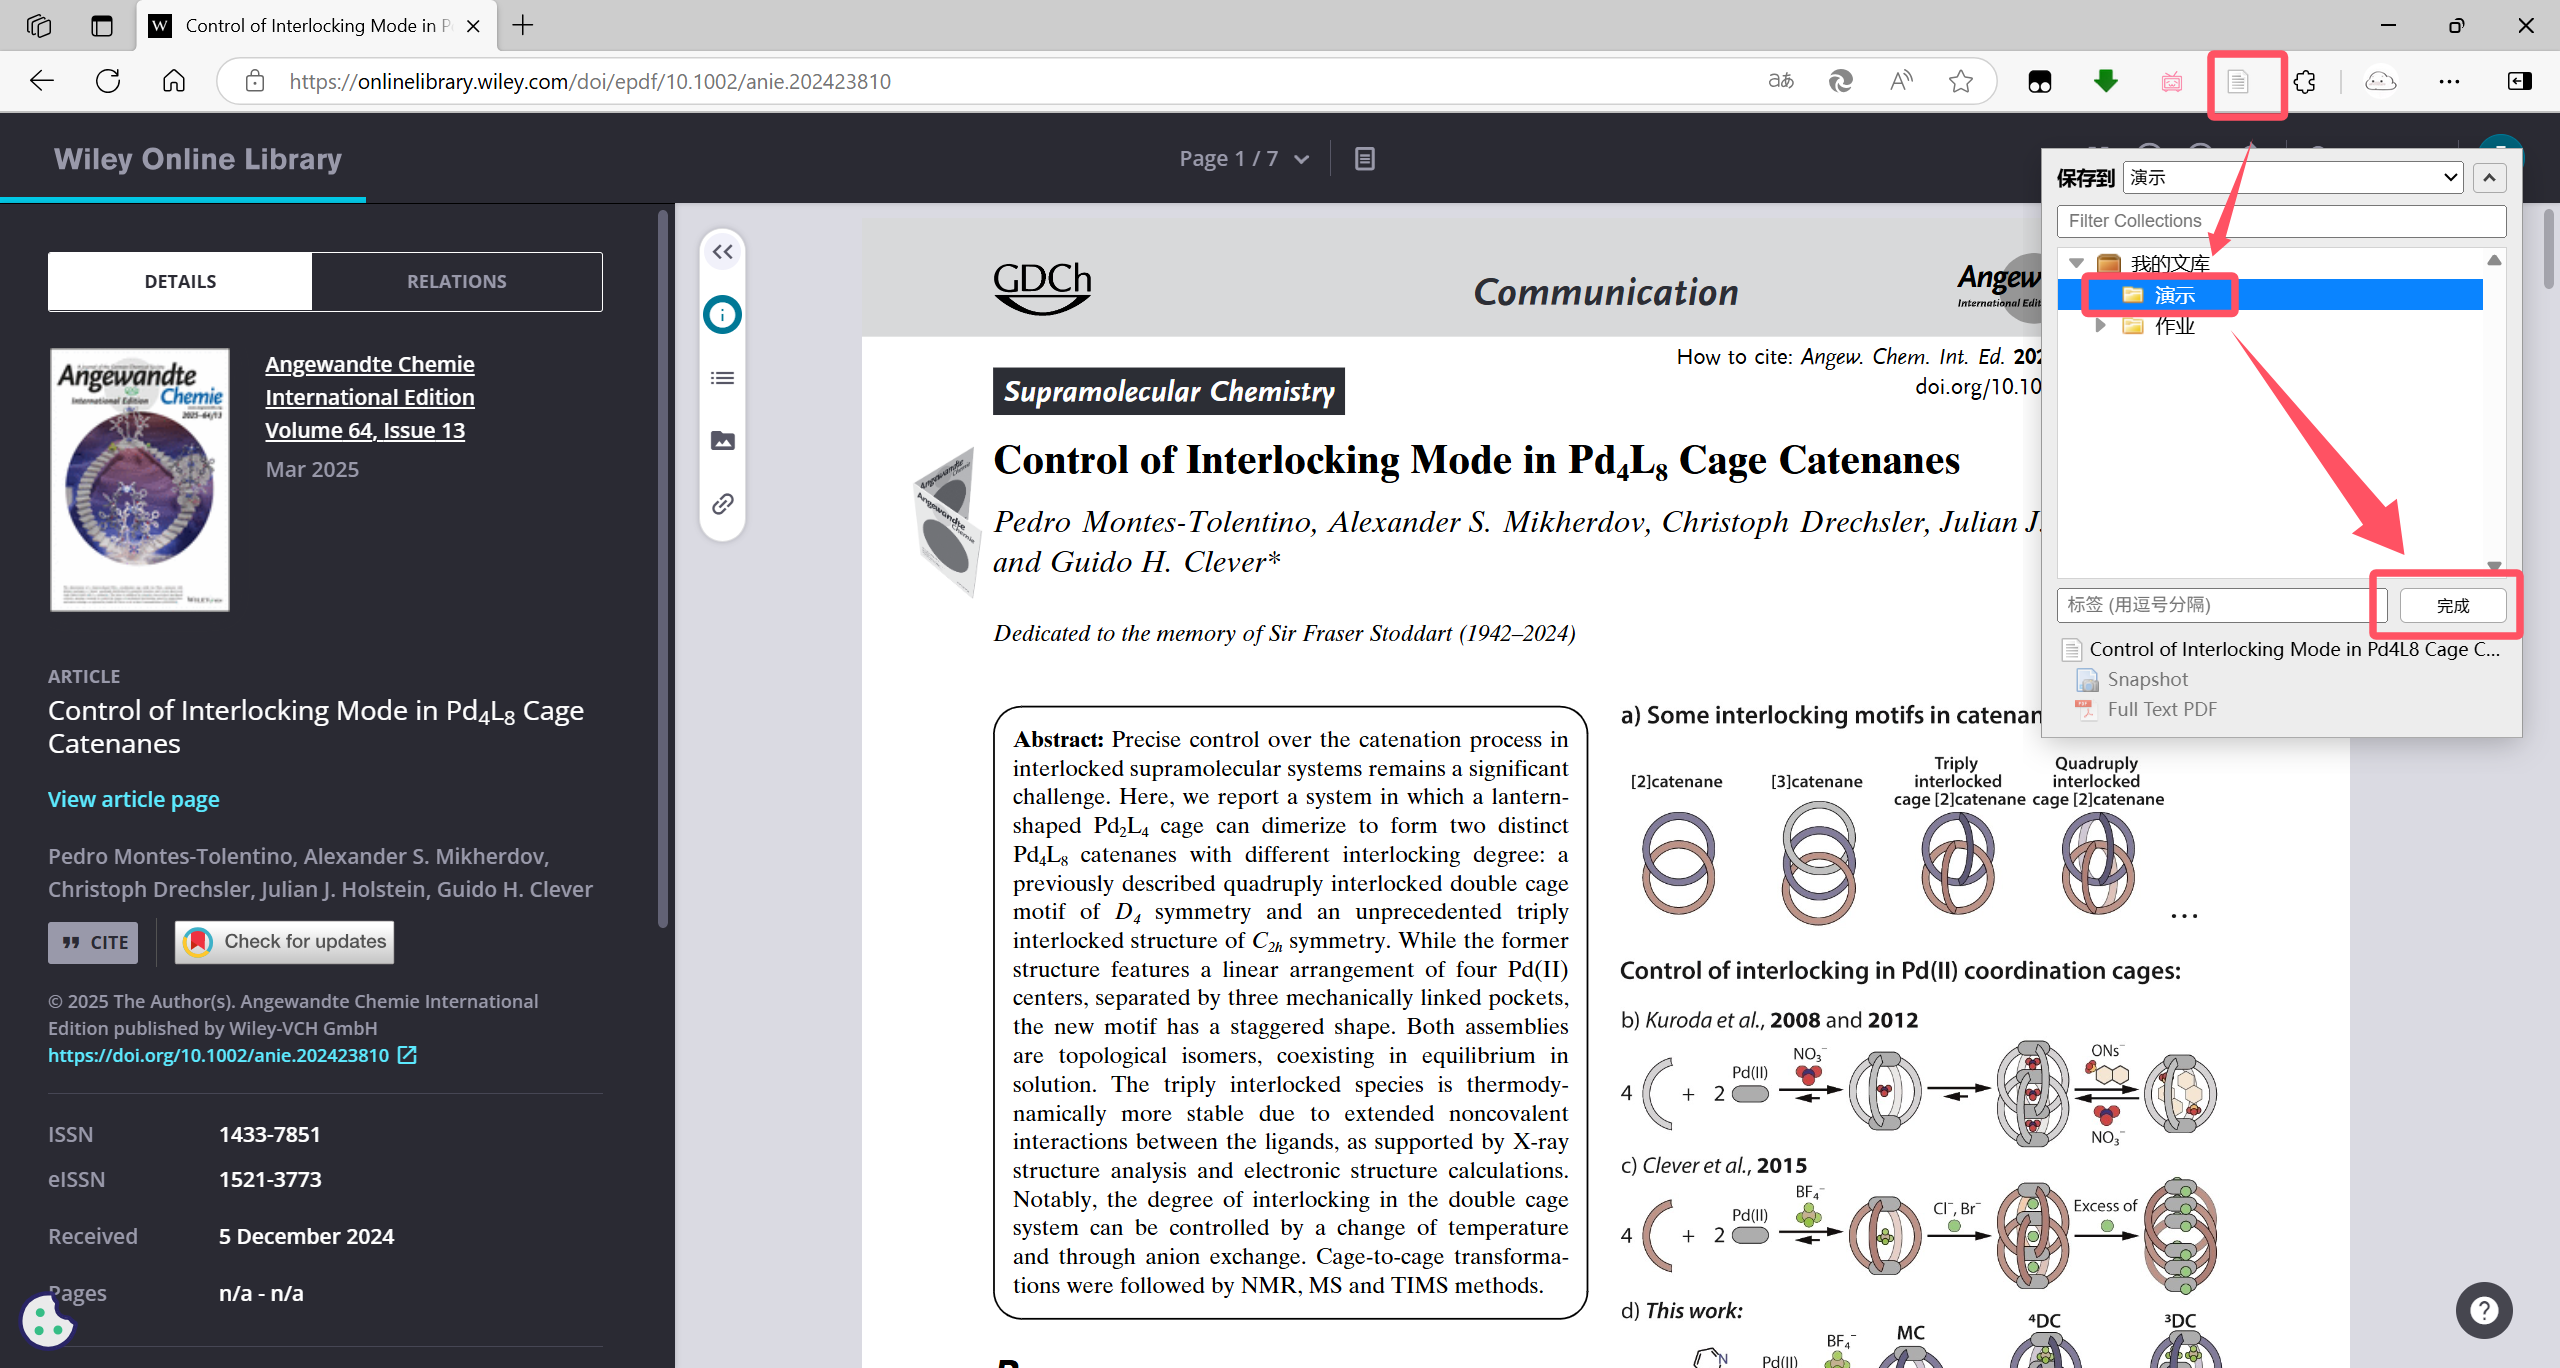
\includegraphics[width=\textwidth]{浏览器导入.png}
      \label{Zotero 3-2}
    \end{subfigure}
    \caption{直接在浏览器导入}
    \label{Zotero 3}
\end{figure}

Zotero具有强大的文献管理功能,配合一些插件也是不错的文献阅读软件。其它操作功能自行探索,不再赘述。

\newpage

\subsection{在Word中插入}
注:若需在其它地方(如PPT)插入参考文献,可在Zotero界面右击所需文件(可多选)或右击左侧文件夹,
选择“用所选条目创建参考文献表”,按提示选择样式,选择复制到剪贴板就可在所需地方粘贴。
但这种方式不如在Word中直接插入智能,不能自动排序或一键更新样式。

在Word中可以方便的使用Zotero插入参考文献,光标定位在要插入的地方,
点击上方Zotero选项卡,点击第一个“插入引用”,每一个文档中首次插入文献会询问引用样式,这个在下一节会讲到。
选择需要的样式后,切换到经典视图,即可插入文献:

\begin{figure}[h]
    \centering
    \captionsetup{font={small, bf}, margin=60pt}
    \begin{subfigure}[c]{0.48\textwidth}
      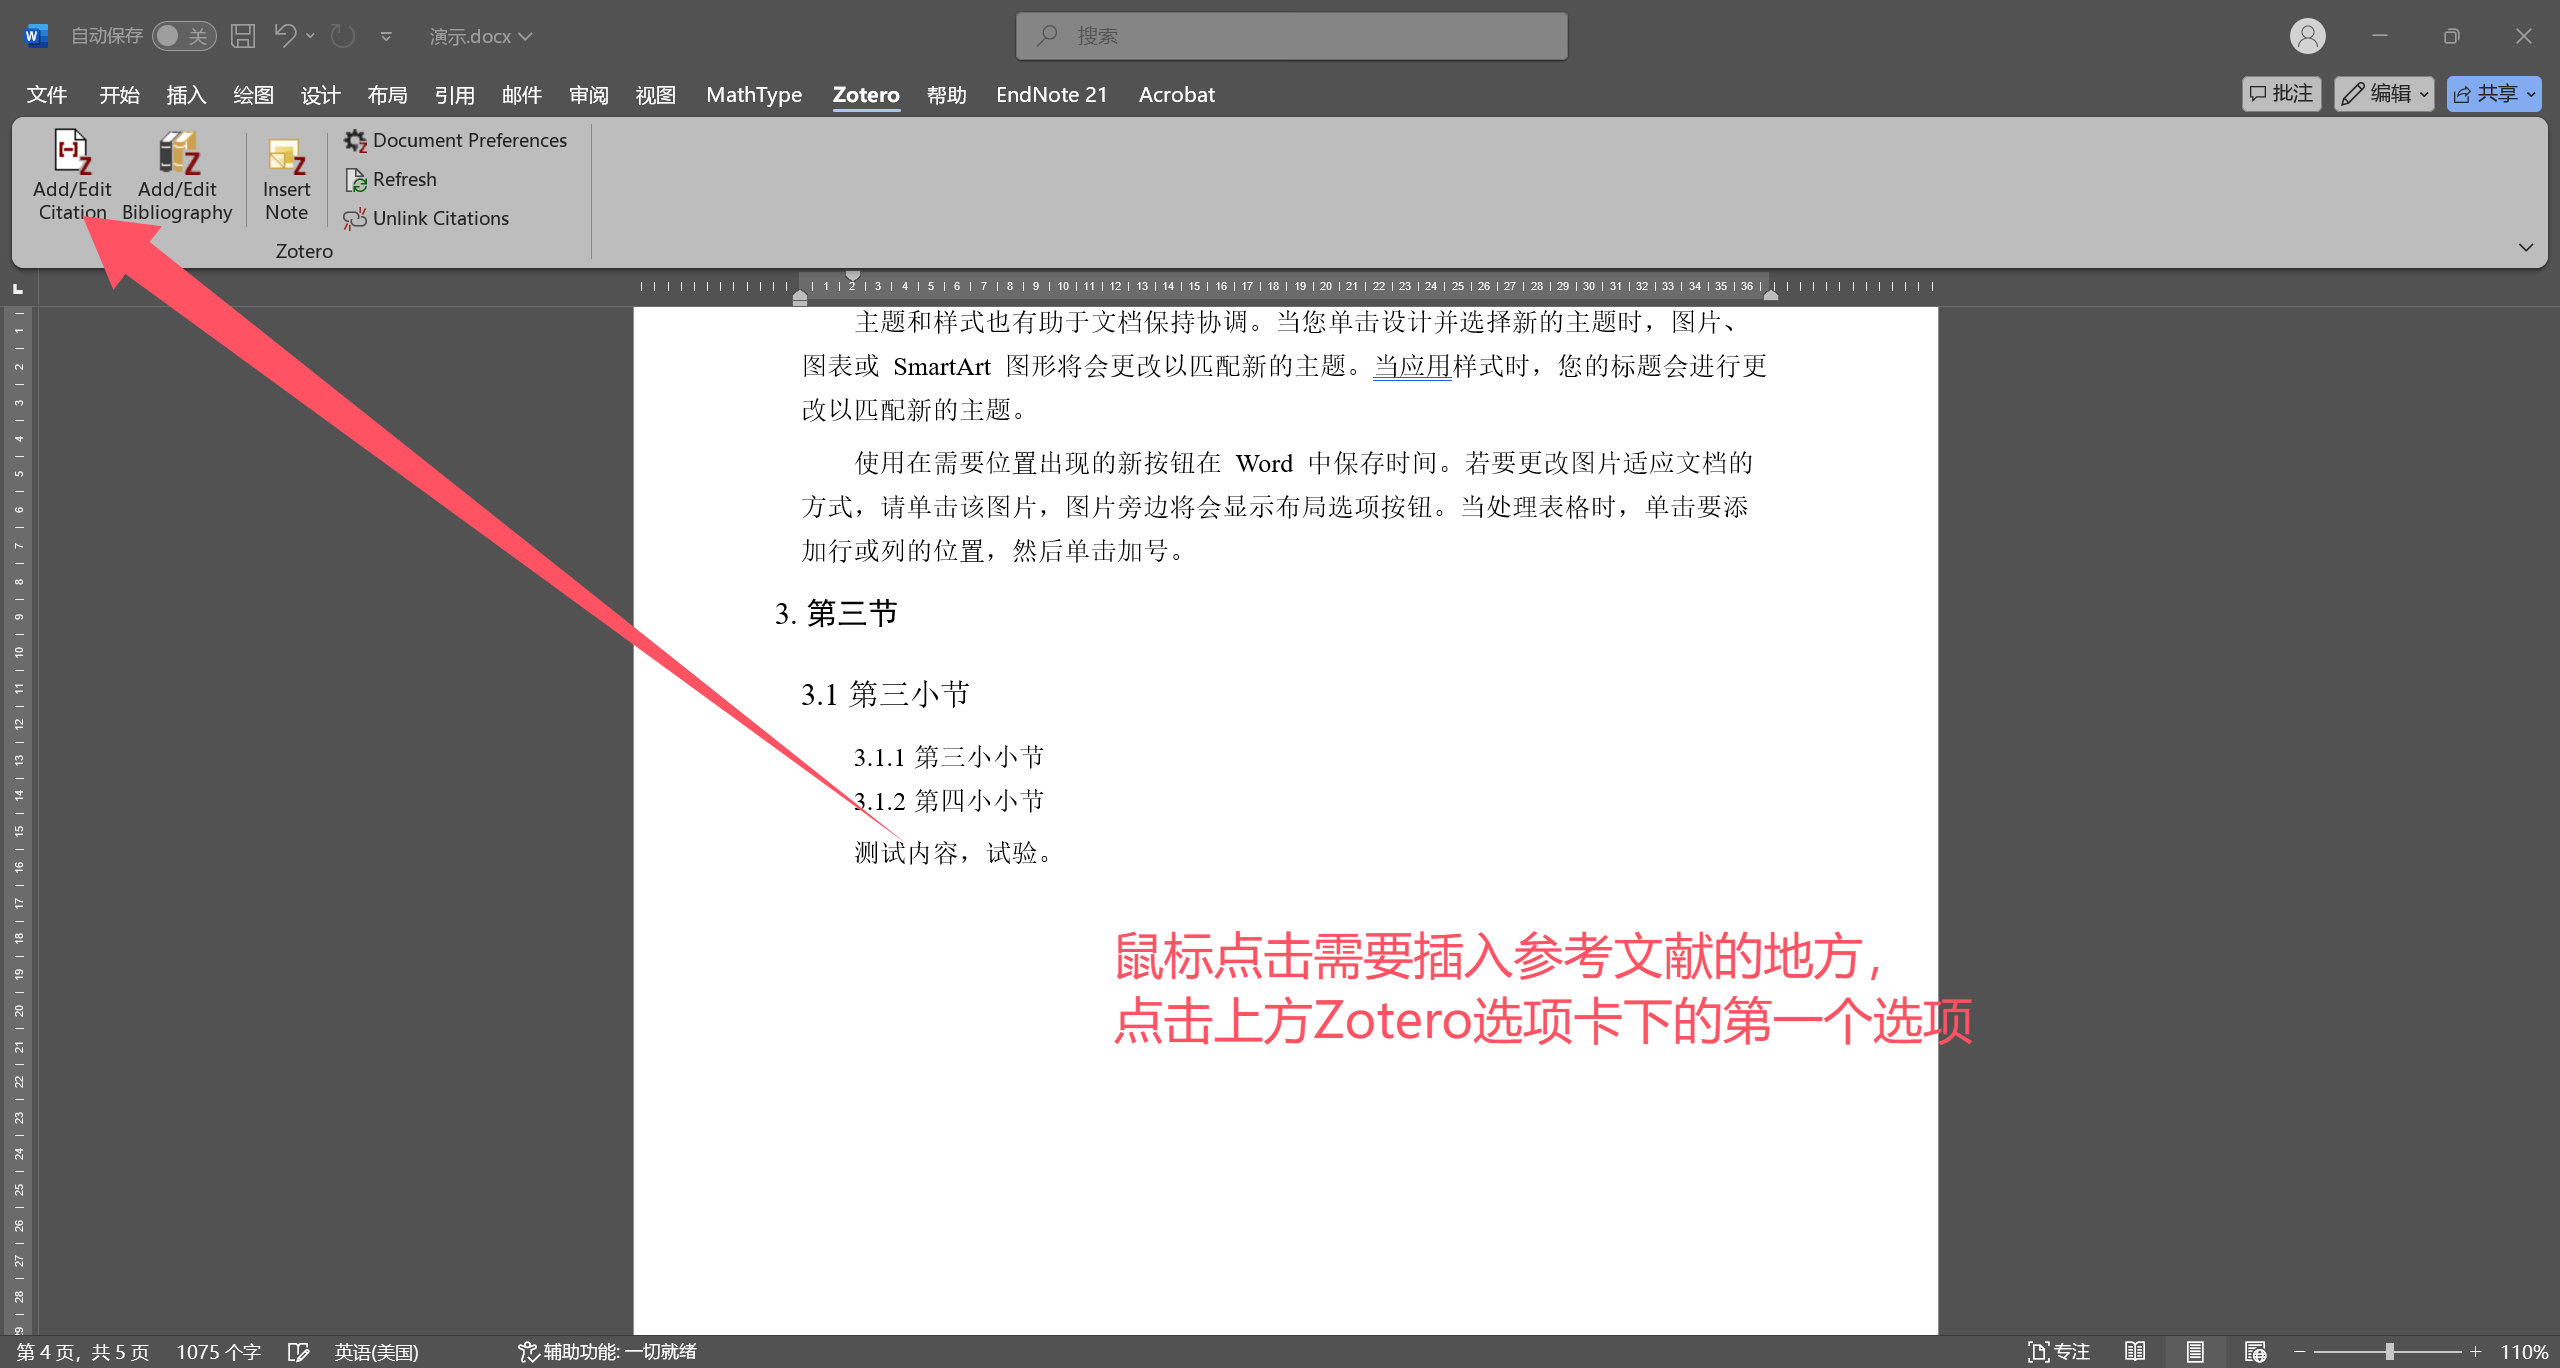
\includegraphics[width=\textwidth]{word使用Zotero-1.png}
      \label{Zotero 4-1}
    \end{subfigure}
    \hfill
    \begin{subfigure}[c]{0.48\textwidth}
      
\includegraphics[width=\textwidth]{word使用Zotero-2.png}
      \label{Zotero 4-2}
    \end{subfigure}
    \hspace{-1em}
    \begin{subfigure}[c]{0.8\textwidth}
        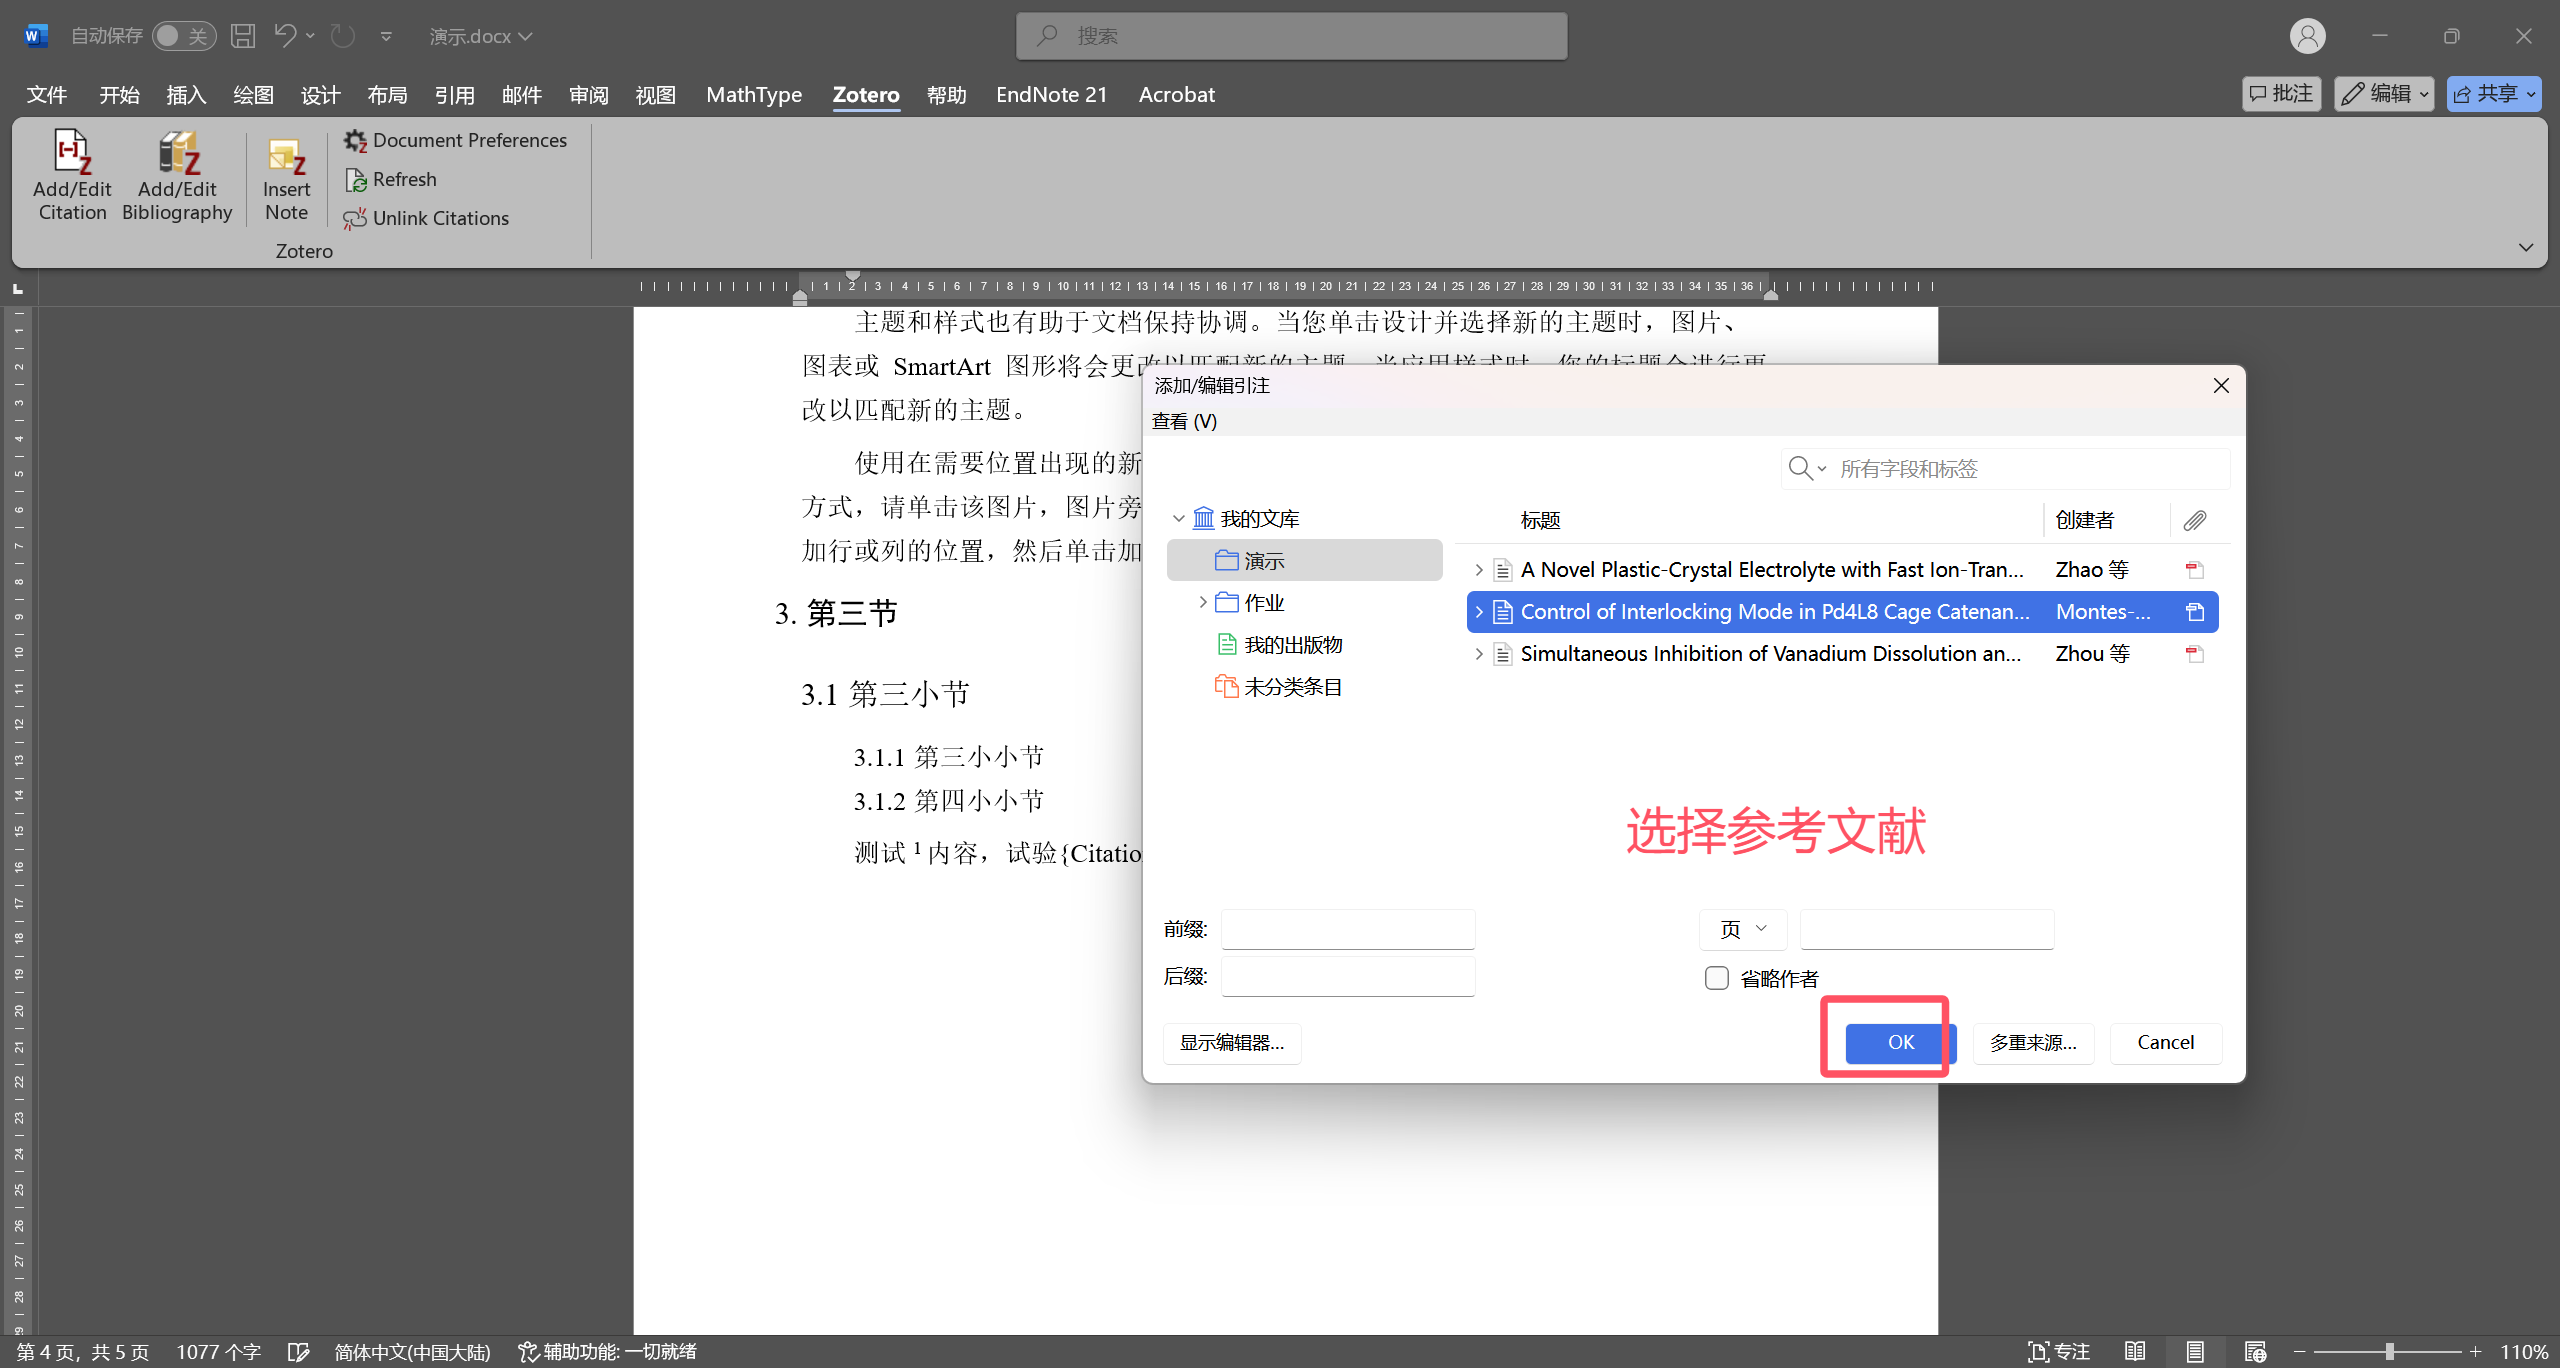
\includegraphics[width=\textwidth]{word使用Zotero-3.png}
        \label{Zotero 4-3}
    \end{subfigure}
    \caption{word使用Zotero}
    \label{Zotero 4}
\end{figure}

还可以插入多个文献,点击插入文献后,在经典视图下,选择“多个来源”,
选择要插入的文献,按右箭头图标进行选择,选择完成后按OK,即可插入:

\newpage

\begin{figure}[h]
    \centering
    \captionsetup{font={small, bf}, margin=60pt}
    \begin{subfigure}[c]{0.48\textwidth}
      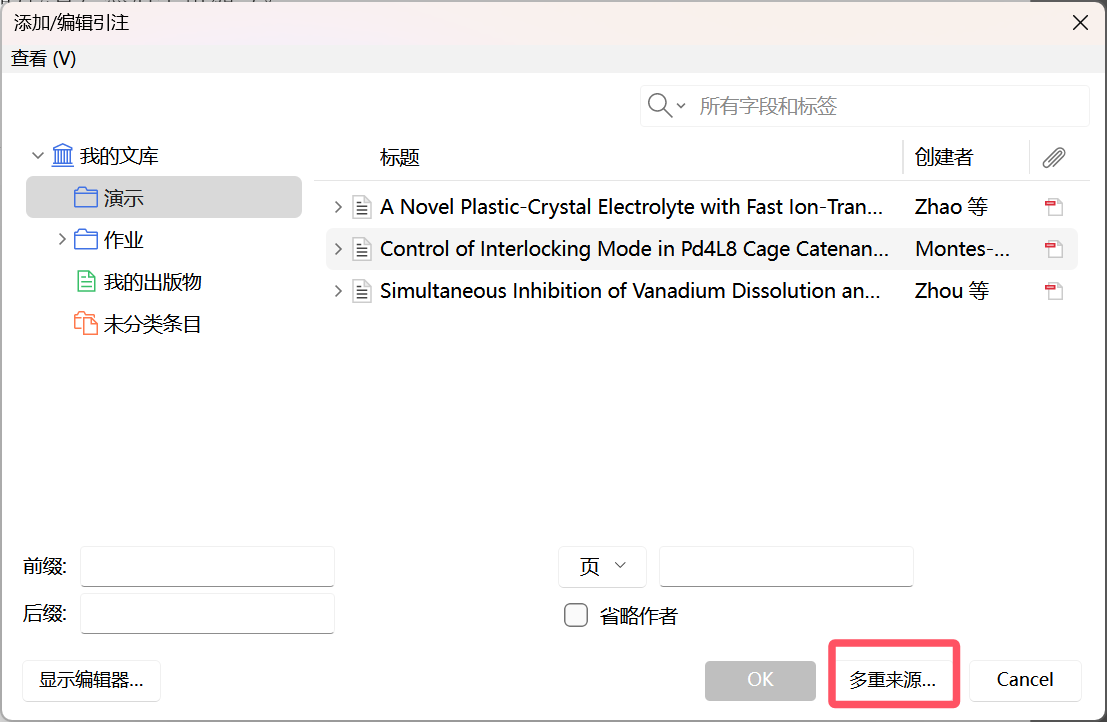
\includegraphics[width=\textwidth]{插入多个文献-2.png}
      \label{Zotero 5-1}
    \end{subfigure}
    \hfill
    \begin{subfigure}[c]{0.48\textwidth}
      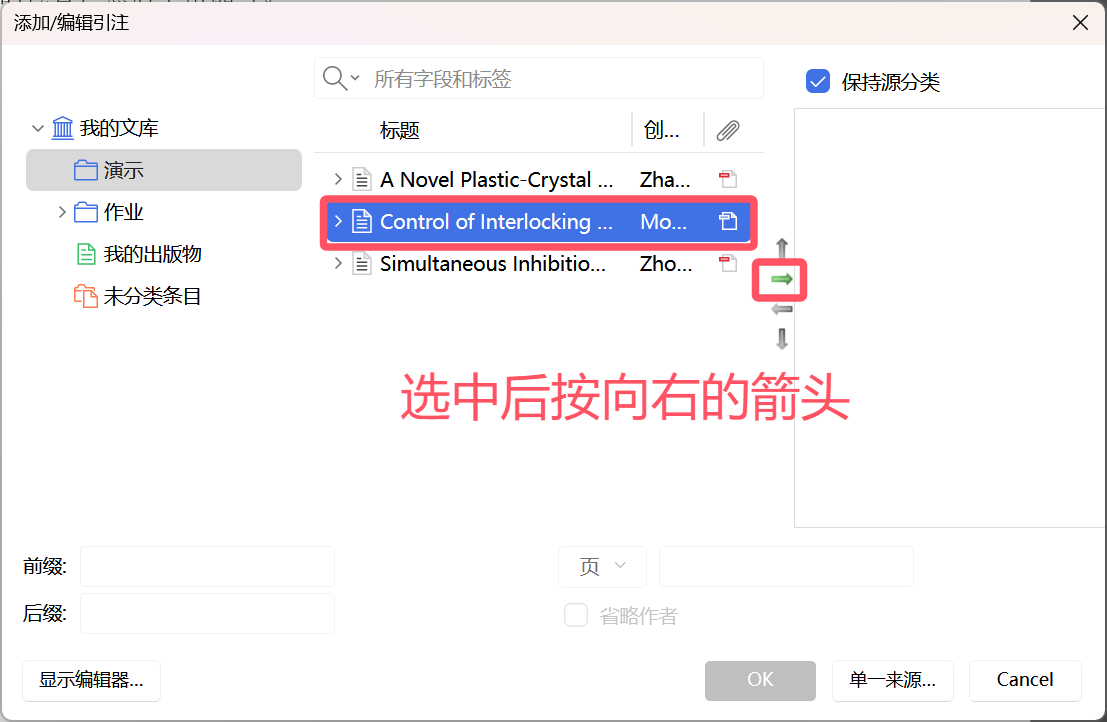
\includegraphics[width=\textwidth]{插入多个文献-1.png}
      \label{Zotero 5-2}
    \end{subfigure}
    \caption{插入多个文献}
    \label{Zotero 5}
\end{figure}

\begin{figure}[!h]
    \centering
    \captionsetup{font={small, bf}, margin=60pt}
    
\includegraphics[width=0.6\textwidth]{插入多个文献效果.png}
    \caption{插入多个文献效果}
    \label{Zotero 6}
\end{figure}

随后在结尾直接点选“Zotero”选项卡下第二个选项“插入书目”,即可直接插入参考文献列表:
\begin{figure}[!h]
    \centering
    \captionsetup{font={small, bf}, margin=60pt}
    
\includegraphics[width=0.6\textwidth]{参考文献.png}
    \caption{参考文献}
    \label{Zotero 7}
\end{figure}

\subsection{参考文献样式}
\subsubsection{选定及更改参考文献样式}
如上节提到,每个Word文档在首次插入文献时会询问参考文献样式,
选择之后,如需更改,可在“Zotero”选项卡下的“Document Preferences”中更改,
若没有立即生效,可点点击“Refresh”手动刷新。
\begin{figure}[!h]
    \centering
    \captionsetup{font={small, bf}, margin=60pt}
    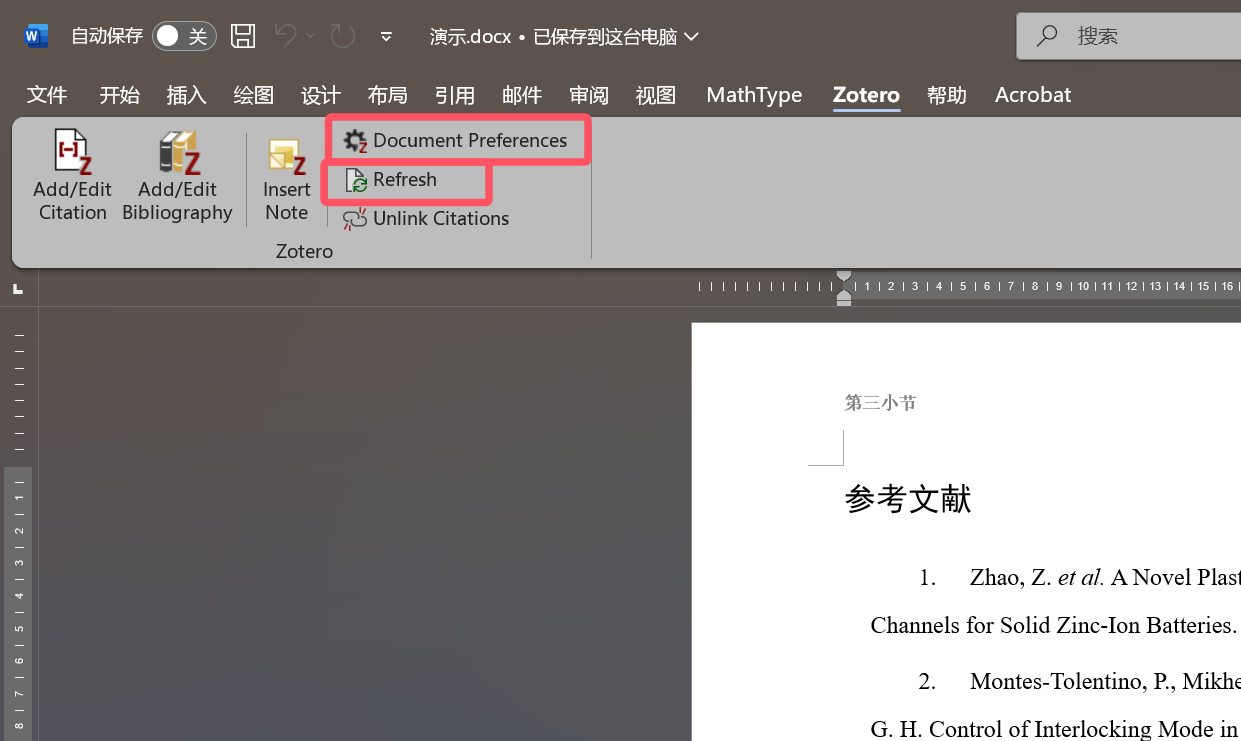
\includegraphics[width=0.6\textwidth]{参考文献样式-1.png}
    \caption{参考文献样式}
    \label{Zotero 8}
\end{figure}

\subsubsection{国标样式}
在国内,我们常用GB/T 7714-2015国标格式,Zotero中需要手动下载。
但在软件内下载的样式有一些缺陷,对双语不友好。
如作者为英文或拼音时,姓名会全部大写,且省略过多作者时显示“等”而不是“et al.”。
针对这些问题,有人整理了更好用的样式,这里提供给大家,可按下图所示安装:

\begin{figure}[!h]
  \centering
  \captionsetup{font={small, bf}, margin=60pt}
  \begin{subfigure}[c]{0.9\textwidth}
      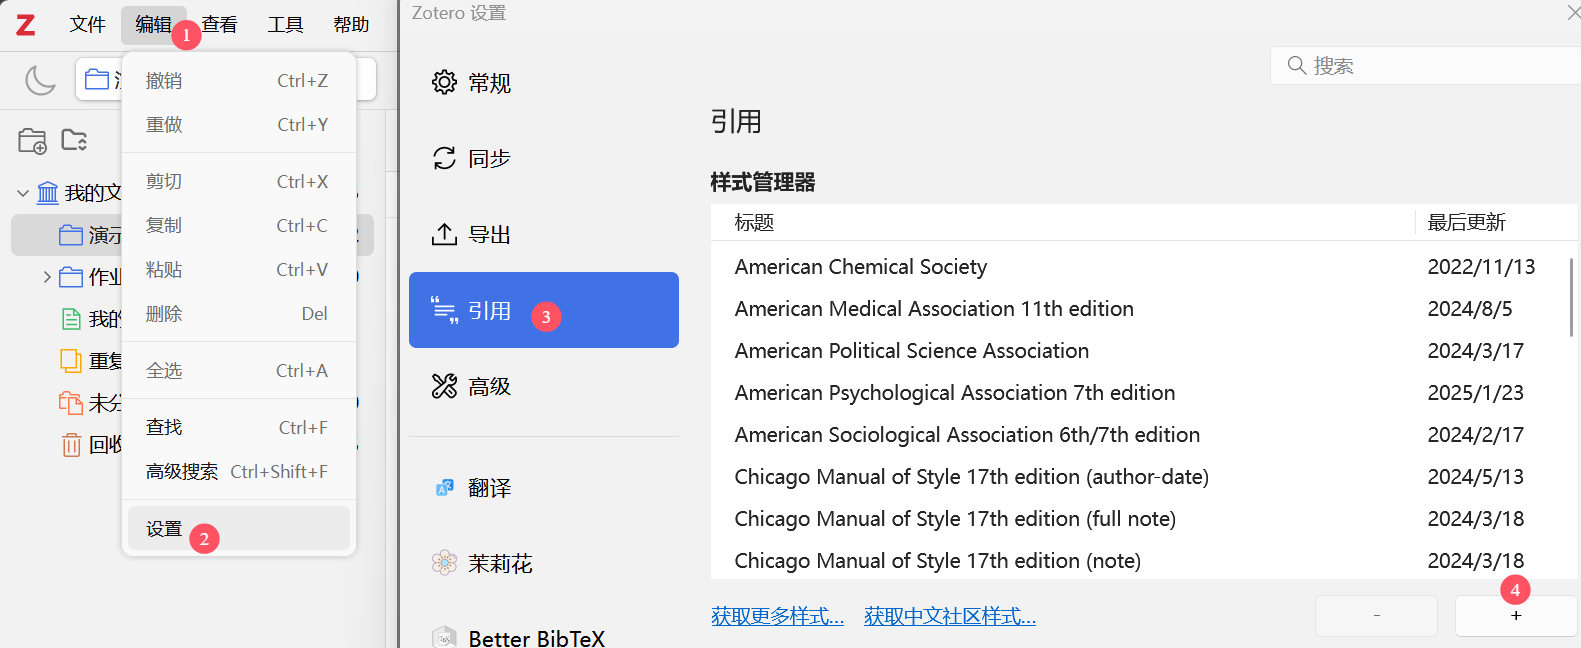
\includegraphics[width=\textwidth]{安装样式-1.png}
      \label{Zotero 9}
  \end{subfigure}
\end{figure}
  \hspace{-1em}

\begin{figure}[h]
  \centering
  \captionsetup{font={small, bf}, margin=60pt}
  \begin{subfigure}[c]{0.48\textwidth}
    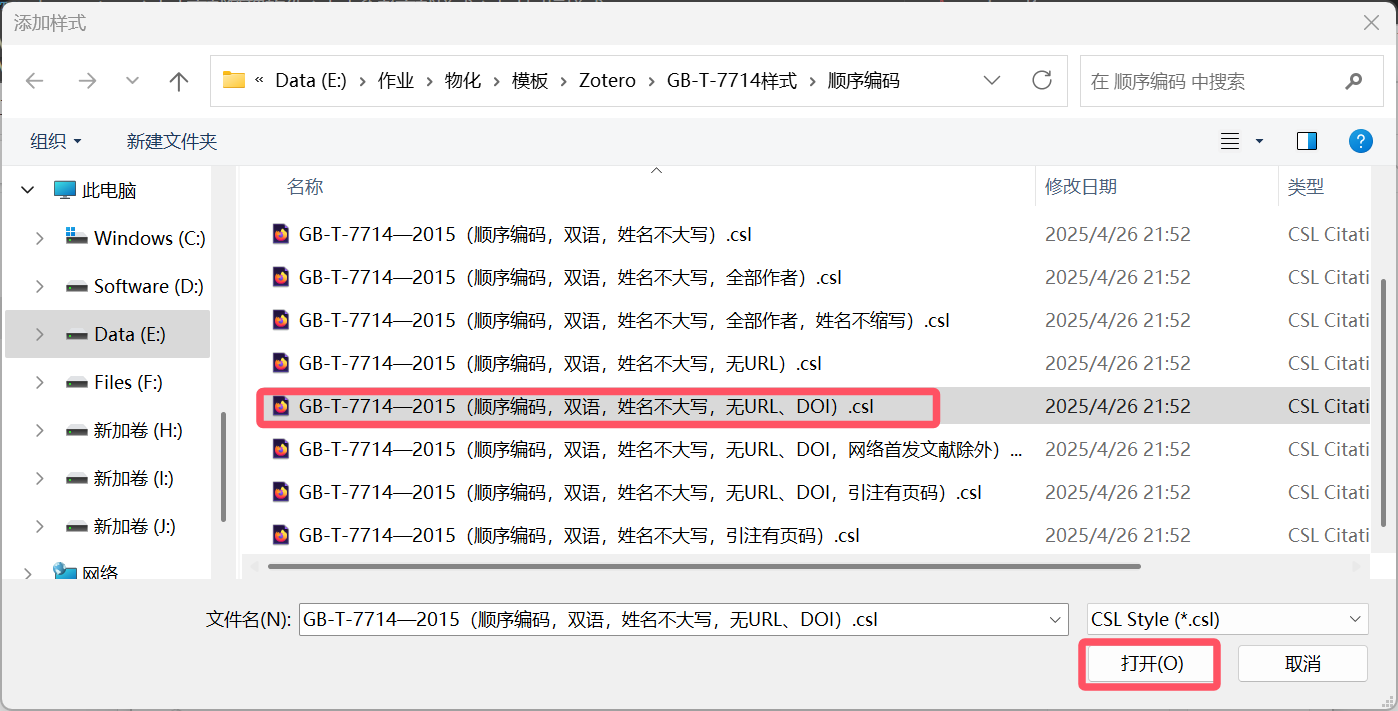
\includegraphics[width=\textwidth]{安装样式-2.png}
    \label{Zotero 10-1}
  \end{subfigure}
  \begin{subfigure}[c]{0.48\textwidth}
    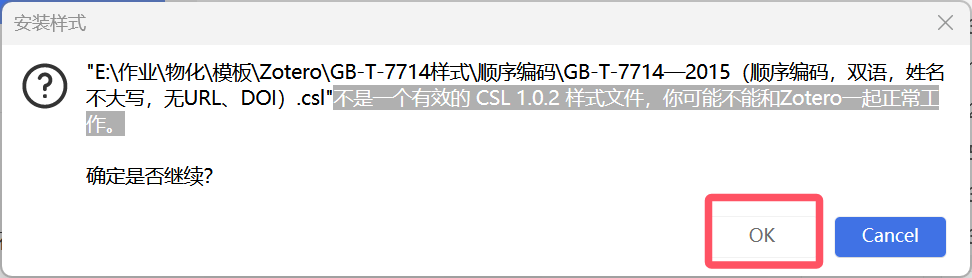
\includegraphics[width=\textwidth]{安装样式-3.png}
    \label{Zotero 10-2}
  \end{subfigure}
  \caption{安装样式}
  \label{Zotero 10}
\end{figure}

我们一般就使用“顺序编码,双语,姓名不大写,无URL、DOI”,其它样式可以按需取用。
安装完成之后,就可以在“Document Preferences”中选择对应样式使用了。

\subsection{插件}
Zotero拥有丰富的插件生态,这里提供两个插件,一个是翻译,在Zotero中查看PDF时,
可以选中文字自动翻译;另一个是茉莉花插件,提供中文文献支持。按如下步骤安装:
\begin{figure}[h]
  \centering
  \captionsetup{font={small, bf}, margin=60pt}
  \begin{subfigure}[c]{0.48\textwidth}
    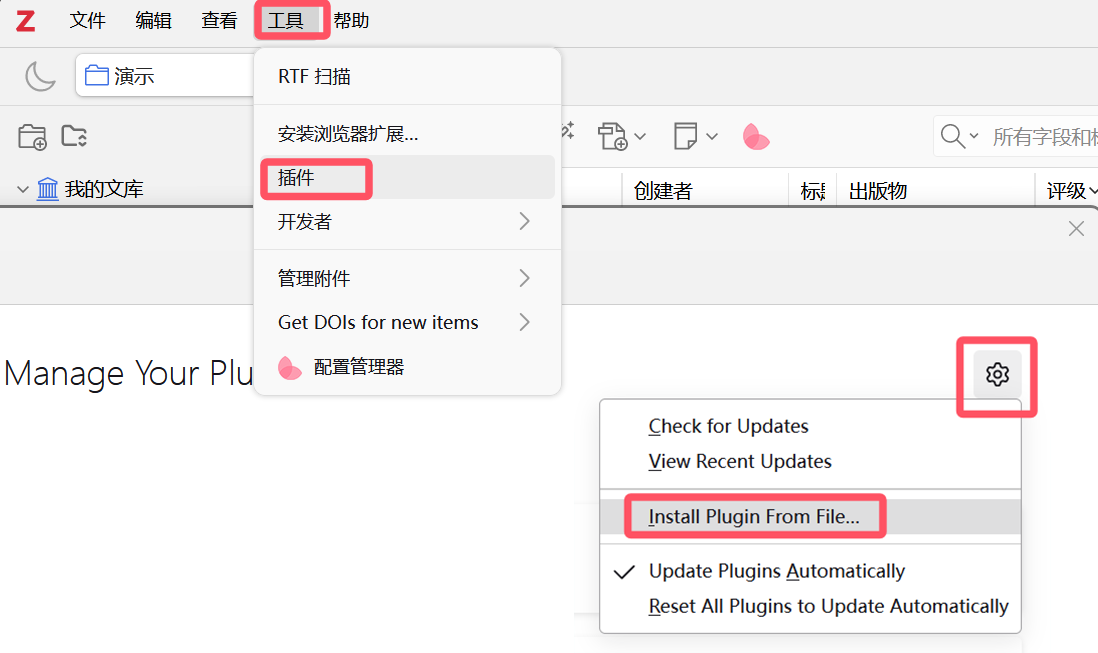
\includegraphics[width=\textwidth]{插件-1.png}
   \label{Zotero 11-1}
  \end{subfigure}
  \hfill
  \begin{subfigure}[c]{0.48\textwidth}
    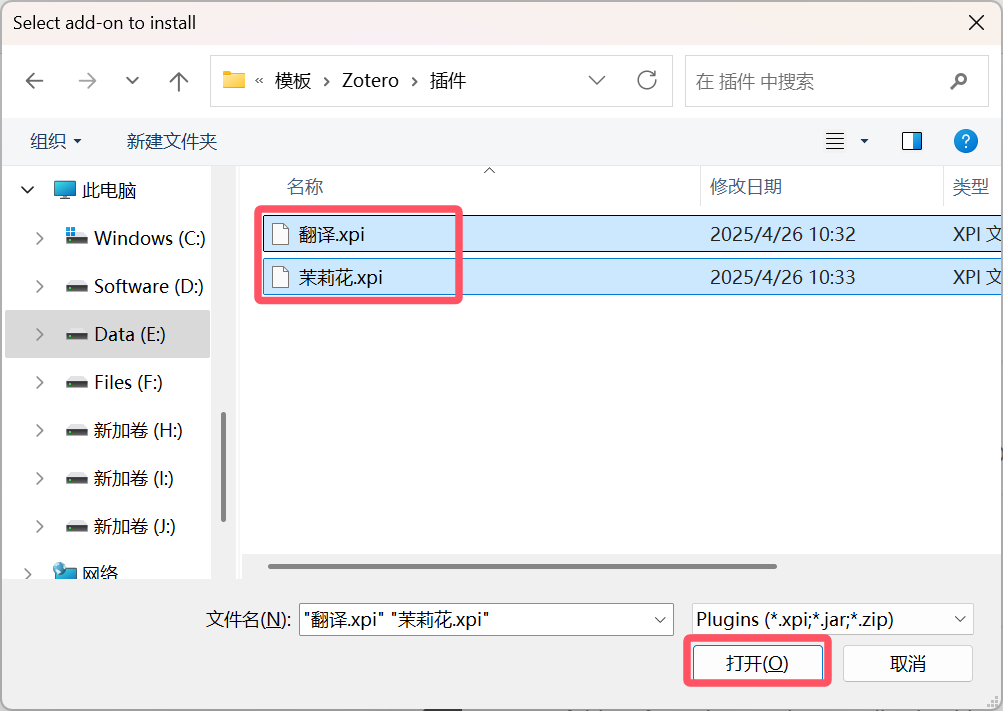
\includegraphics[width=\textwidth]{插件-2.png}
    \label{Zotero 11-2}
  \end{subfigure}
  \caption{插件}
  \label{Zotero 11}
\end{figure}

其他插件可以在\textbf{\textcolor{blue}{\href{https://zotero-chinese.com/plugins/}{Zotero中文社区插件}}}找到,安装方法类似。
